% Elsevier CAS-DC-compatible results section for the CGPO manuscript.
% The structure follows the local Swarm and Evolutionary Computation UAV papers:
% overall performance, rankings/statistics, convergence, PF/path visualization,
% ablation, runtime/safety, and final discussion.
%
% Required source artifacts for the reduced manuscript:
% - results/cgpo_swec_matched_40x500_5run/metrics/benchmark_metrics_summary.csv
% - results/paper_artifacts/cgpo-swec/tables/cgpo_matched_overall_40x500_5run.csv
% - results/paper_artifacts/cgpo-swec/tables/cgpo_matched_pairwise_40x500_5run.csv
% - results/paper_artifacts/cgpo-swec/tables/cgpo_matched_rank_40x500_5run.csv
% - results/cgpo_swec_ablation_40x500_1run/metrics/benchmark_metrics_summary.csv
%
% Do not use initialization-smoke values for paper claims.
% Preamble requirement: \usepackage{booktabs}

\section{Results and discussion}
\label{sec:results}

This section reports the experimental evidence for CGPO on the constrained multi-UAV benchmark. Following the evaluation style used in recent \textit{Swarm and Evolutionary Computation} UAV path-planning studies, the analysis begins with aggregate hypervolume and statistical comparisons, then examines scenario-level behavior, convergence, Pareto-front and path visualizations, runtime, safety diagnostics, reference-code comparisons, and mechanism ablations. The objective is not only to rank optimizers, but also to determine whether graph-derived selection pressure and fleet-aware variation improve feasible multi-objective search without hiding constraint violations behind a repair stage.

\subsection{Overall performance analysis}
\label{subsec:overall-performance}

Table~\ref{tab:overall-performance} summarizes the reduced matched paper comparison over the city, mountain, and suburban fleet-three scenarios. Values are aggregated over five runs per scenario with population 40 and 500 generations. UAV-specialized and MAPF-style methods remain outside this reduced run and should not be used for headline numerical claims until they are fairly wired into the same protocol.

\begin{table*}[t]
\centering
\caption{Reduced matched fleet performance across \texttt{c\_100\_uav3}, \texttt{m\_100\_uav3}, and \texttt{s\_120\_uav3}. HV and runtime are averaged over scenario-level means; each scenario has five runs.}
\label{tab:overall-performance}
\scriptsize
\setlength{\tabcolsep}{3pt}
\begin{tabular*}{\textwidth}{@{\extracolsep{\fill}}p{0.18\textwidth}p{0.16\textwidth}ccccc}
\toprule
Role & Method & Feasible ratio $\uparrow$ & HV $\uparrow$ & IGD+ $\downarrow$ & Conflict rate $\downarrow$ & Runtime (s) $\downarrow$ \\
\midrule
Proposed & \texttt{CGPO} & 1.0000 & 0.1728 & 0.0981 & 0.0000 & 76.4872 \\
Canonical MOEA baseline & \texttt{NSGA-II} & 0.0000 & 0.0000 & n/a & 0.0000 & 25.7643 \\
Decomposition baseline & \texttt{MOEA/D} & 0.6000 & 0.0834 & 0.2382 & 0.0000 & 24.0834 \\
UAV PSO baseline & \texttt{NMOPSO} & 0.0000 & 0.0000 & n/a & 0.0001 & 26.2931 \\
\bottomrule
\end{tabular*}
\end{table*}

CGPO is the only method that returns feasible populations in every matched run and has the highest reduced-protocol HV. MOEA/D is the strongest non-CGPO baseline, but it fails the city fleet-three case and internally uses 35 NBI weight vectors for the requested population of 40. NSGA-II and NMOPSO produce no feasible final populations under the same budget after feasible-mask filtering.

\subsection{Ranking and statistical comparison}
\label{subsec:ranking-statistics}

Table~\ref{tab:rank-statistics} reports the reduced-protocol scenario-level HV rank and the primary matched run-level statistical evidence against CGPO. The tests are matched by problem and run index; MOEA/D has 14 matched final-HV entries because one mountain entry is unavailable.

\begin{table*}[t]
\centering
\caption{Average scenario-level HV rank and matched run-level comparison against CGPO. Lower rank is better.}
\label{tab:rank-statistics}
\small
\setlength{\tabcolsep}{4pt}
\begin{tabular*}{\textwidth}{@{\extracolsep{\fill}}lccccc}
\toprule
Comparison target & Average rank & Metric & Matched $n$ & Holm-adjusted $p$ & CGPO W/T/L \\
\midrule
\texttt{CGPO} & 1.0 & HV & -- & -- & -- \\
\texttt{MOEA/D} & 2.0 & HV & 14 & $9.16\times10^{-5}$ & 14/0/0 \\
\texttt{NMOPSO} & 3.0 & HV & 15 & $9.16\times10^{-5}$ & 15/0/0 \\
\texttt{NSGA-II} & 4.0 & HV & 15 & $9.16\times10^{-5}$ & 15/0/0 \\
\bottomrule
\end{tabular*}
\end{table*}

CGPO ranks first in all three reduced fleet-three scenario groups. The matched run-level tests give a consistent win profile against MOEA/D, NSGA-II, and NMOPSO, supporting a reduced-budget claim against these three baselines.

\subsection{Scenario-wise and fleet-size analysis}
\label{subsec:scenario-wise}

Figure~\ref{fig:scenario-fleet-hv} summarizes the data-derived reduced comparison. It shows the mean HV, feasible ratio, and runtime columns used in the main manuscript table.

\begin{figure*}[t]
\centering
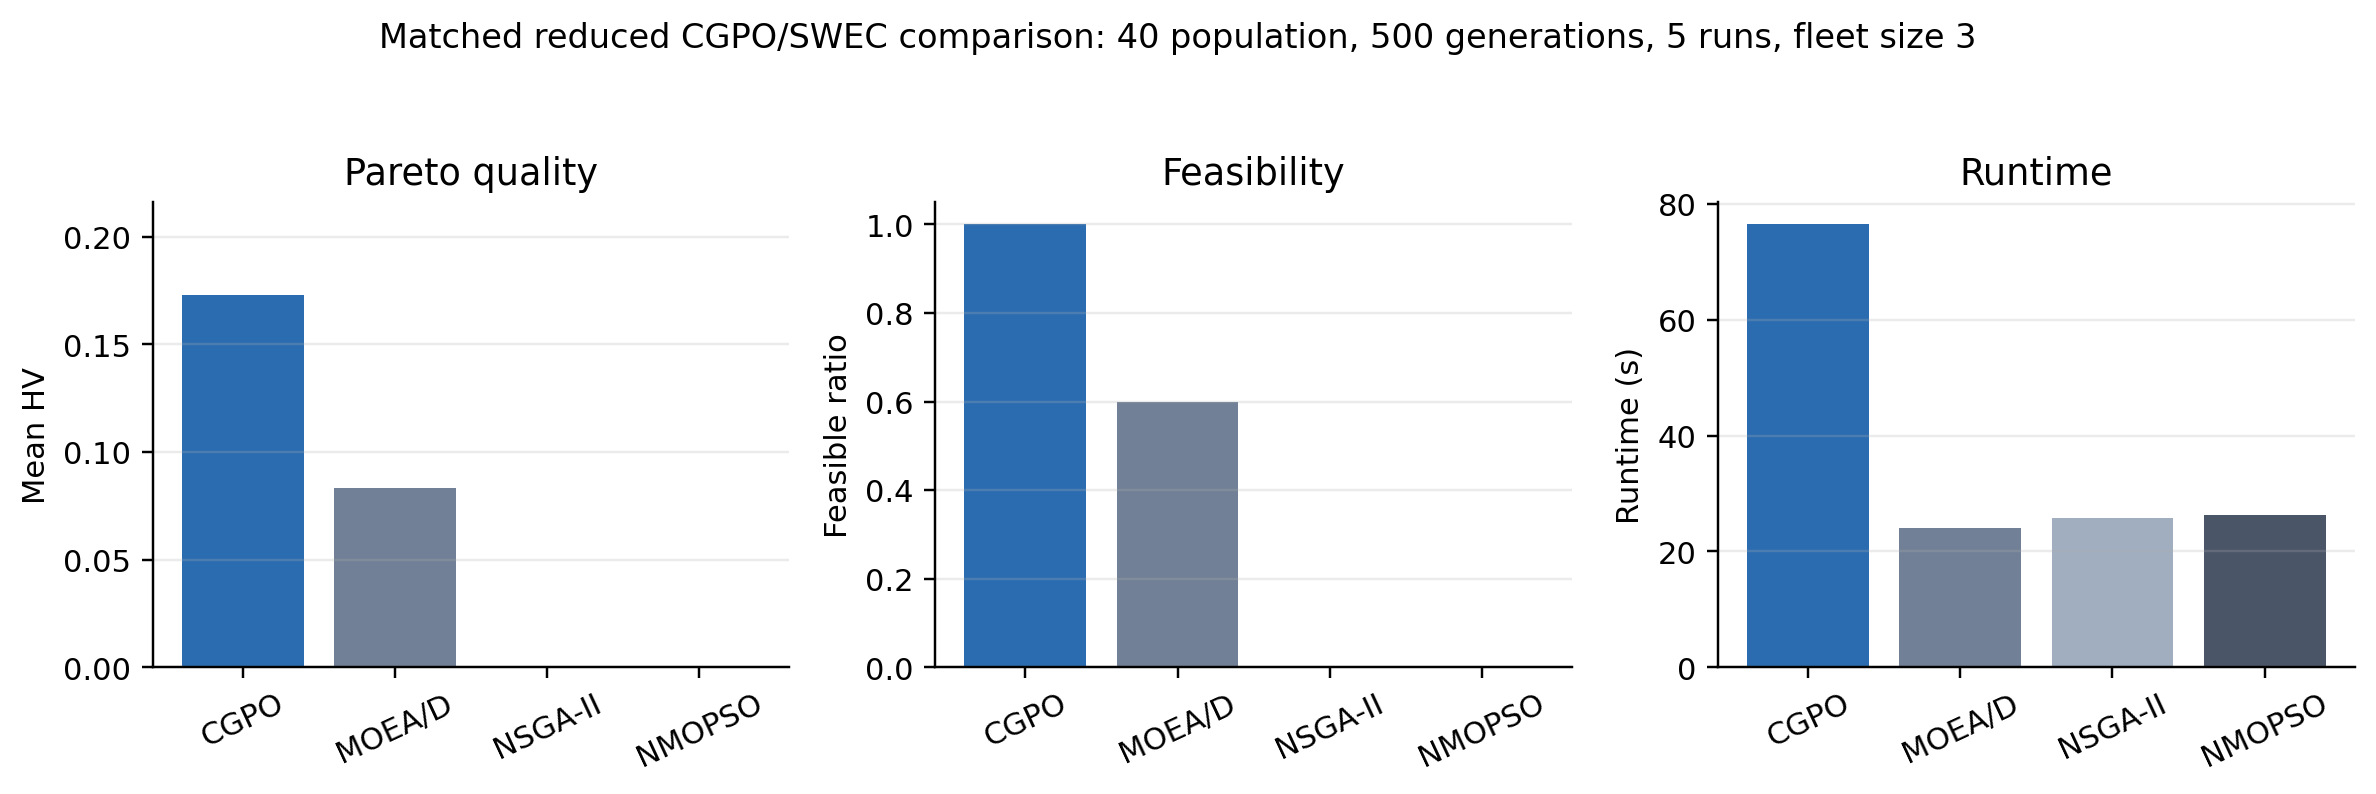
\includegraphics[width=0.96\textwidth]{figures/cgpo_matched_results_40x500_5run.png}
\caption{Reduced matched result summary generated from \texttt{results/cgpo\_swec\_matched\_40x500\_5run/metrics/benchmark\_metrics\_summary.csv}.}
\label{fig:scenario-fleet-hv}
\end{figure*}

The reduced run covers only fleet size 3, so it cannot support claims about scaling from one to five UAVs. The separate inspection table in the main manuscript provides descriptive three- and eight-UAV CGPO evidence, but that evidence is not a matched baseline comparison.

\subsection{Convergence behavior}
\label{subsec:convergence}

Convergence curves provide information that the final HV table cannot show. Figure~\ref{fig:convergence} should plot median HV over generations for representative city, mountain, and suburban cases. The main patterns to report are convergence speed, late-stage improvement, stagnation, and variance across runs.

\begin{figure*}[t]
\centering
\fbox{\parbox[c][38mm][c]{0.92\textwidth}{\centering Placeholder for convergence curves using recorded metric intervals. Curves should compare CGPO with the strongest non-CGPO family representatives.}}
\caption{Convergence behavior on representative scenarios. Curves should use the same metric interval and run budget as the paper-grade protocol.}
\label{fig:convergence}
\end{figure*}

If CGPO converges more slowly but reaches a better final feasible HV, the method should be described as investing additional computation in constraint-guided exploration. If CGPO converges quickly but stagnates, the discussion should connect this to the pressure-field or variation behavior. This style follows the reference papers' practice of using convergence plots to explain table-level rankings.

\subsection{Pareto-front and trajectory visualization}
\label{subsec:pf-path-visualization}

Figure~\ref{fig:pf-path} should combine representative Pareto-front distributions with 3D trajectory visualizations. The Pareto-front panel should show whether CGPO improves convergence, spread, or boundary coverage. The path panel should show whether the selected compromise solutions satisfy terrain clearance, smoothness, and inter-UAV separation in visually interpretable cases.

\begin{figure*}[t]
\centering
\fbox{\parbox[c][42mm][c]{0.92\textwidth}{\centering Placeholder for representative Pareto fronts and 3D fleet paths. Use one urban, one suburban, and one mountainous case.}}
\caption{Representative Pareto fronts and UAV trajectories. Visualizations should be selected from median or best-compromise runs and must not replace the aggregate statistical results.}
\label{fig:pf-path}
\end{figure*}

The visual analysis should be practical rather than decorative. A useful CGPO trajectory should avoid terrain and fleet conflicts while maintaining competitive path length and smoothness. If a path looks visually safe but the diagnostic table reports constraint failures, the numeric safety result takes priority.

\subsection{Runtime and safety diagnostics}
\label{subsec:runtime-safety}

Table~\ref{tab:runtime-safety} reports runtime and mission-level safety diagnostics. This table is necessary because graph construction, pressure-field computation, and fleet-aware variation add computational cost. It also prevents the paper from claiming quality improvements that come from unsafe solutions.

\begin{table*}[t]
\centering
\caption{Runtime and safety diagnostics for the reduced matched fleet comparison.}
\label{tab:runtime-safety}
\small
\setlength{\tabcolsep}{4pt}
\begin{tabular*}{\textwidth}{@{\extracolsep{\fill}}lccccc}
\toprule
Method group & Runtime (s) $\downarrow$ & HV/sec $\uparrow$ & Run success $\uparrow$ & Min. clearance $\uparrow$ & Max. turn angle $\downarrow$ \\
\midrule
\texttt{CGPO} & 76.4872 & 0.0023 & 1.0000 & 1.3598 & 74.9551 \\
Best non-CGPO overall (\texttt{MOEA/D}) & 24.0834 & 0.0035 & 0.6000 & -104.4030 & 79.6143 \\
Fastest baseline (\texttt{MOEA/D}) & 24.0834 & 0.0035 & 0.6000 & -104.4030 & 79.6143 \\
\bottomrule
\end{tabular*}
\end{table*}

CGPO is slower than the three reduced baselines, but it is the only method with full feasibility and positive feasible-mask HV across all three scenarios. The discussion should therefore frame the result as a quality-safety trade-off, not as a runtime win.

\subsection{Single-UAV reference-code context}
\label{subsec:reference-code}

Table~\ref{tab:reference-code} records the publication gap for specialized single-UAV reference-code methods. These methods are important context, but they were not part of the completed reduced matched run and should remain out of headline numerical claims.

\begin{table*}[t]
\centering
\caption{Single-UAV reference-code comparison status.}
\label{tab:reference-code}
\small
\setlength{\tabcolsep}{4pt}
\begin{tabular*}{\textwidth}{@{\extracolsep{\fill}}lccccc}
\toprule
Algorithm & Feasible ratio $\uparrow$ & HV $\uparrow$ & IGD+ $\downarrow$ & Runtime (s) $\downarrow$ & Interpretation \\
\midrule
\texttt{CGPO} & -- & -- & -- & -- & not run in reduced single-UAV reference protocol \\
\texttt{MOEA-2DE} & -- & -- & -- & -- & deferred fair-wiring / import \\
\texttt{EMMOP} & -- & -- & -- & -- & deferred fair-wiring / import \\
\bottomrule
\end{tabular*}
\end{table*}

If a specialized single-UAV method outperforms CGPO, the discussion should state that single-UAV heuristic operators remain strong in their native scope. The main CGPO claim should still be judged on the fleet-constrained benchmark and mechanism ablation. Offline methods, including L-SHADE-CDP, C-TAEA, GCNMOEA, MO-MFEA-II, MOEAD-AWA-ASTAR, and external methods that are not yet wired locally, should be discussed qualitatively or reported only after fair implementation or result import.

\subsection{Ablation study}
\label{subsec:ablation}

The ablation study tests whether the three-mechanism CIG/PPF/OVO stack of the lean CGPO contributes to the observed performance. Table~\ref{tab:ablation} reports the full method, an all-disabled \texttt{random\_only} lower bound, three single-mechanism removals, and an additional surgical variant that disables only the OVO fleet-coordination pass. This follows the SWEC style of pairing overall performance with component-removal evidence. Removed prototype variants based on explicit repair, graph-guided feasibility projection, constructive priors, and matched CGPO hybrids are not part of the active paper protocol.

\begin{table*}[t]
\centering
\caption{Lean CGPO three-mechanism ablation on \texttt{s\_120\_uav3} using population 40, 500 generations, and one run per variant. Values are descriptive single-run results.}
\label{tab:ablation}
\small
\setlength{\tabcolsep}{4pt}
\begin{tabular*}{\textwidth}{@{\extracolsep{\fill}}lccccc}
\toprule
Variant & Removed mechanism & Feasible ratio & HV & IGD+ & Decision \\
\midrule
\texttt{CGPO\_full} & none & 1.0 & 0.4540 & 0.0514 & reference \\
\texttt{CGPO\_random\_only} & all three (CIG, PPF, OVO) & 1.0 & 0.3676 & 0.1927 & lower HV, higher IGD+ \\
\texttt{CGPO\_no\_cig\_edge\_coupling} & CIG edge coupling & 1.0 & 0.4590 & 0.0480 & descriptive tie/improvement \\
\texttt{CGPO\_no\_ppf\_pressure} & PPF pressure & 1.0 & 0.4639 & 0.0358 & descriptive improvement \\
\texttt{CGPO\_no\_ovo\_variation} & OVO variation operator & 1.0 & 0.3182 & 0.2129 & lower HV, higher IGD+ \\
\texttt{CGPO\_no\_ovo\_fleet\_coordination} & OVO fleet-coordination pass & 1.0 & 0.4479 & 0.0446 & descriptive tie \\
\bottomrule
\end{tabular*}
\end{table*}

The ablation interpretation is conservative. If removing a component does not degrade performance or safety, that component is described as conditionally useful or as a simplification target. The paper claims a three-part mechanism only if the evidence supports all three parts; if a single-mechanism removal does not change the external metrics, the discussion treats that mechanism as inspectable but not empirically necessary.

\subsection{Trace analysis}
\label{subsec:trace}

Figure~\ref{fig:trace-dynamics} links the internal CGPO signals to the ablation results. The figure should show CIG mean tension and pairwise/smoothing edge counts, PPF feasibility pressure or pressure entropy, and OVO perturbation scale and coordinated-cluster count, for the full method and the degradation variants. Projection-related trace fields remain zero-valued compatibility columns in the artifact schema and are not interpreted as active mechanisms.

\begin{figure*}[t]
\centering
\fbox{\parbox[c][38mm][c]{0.92\textwidth}{\centering Placeholder for CGPO trace dynamics. Source: \texttt{results/cgpo\_swec\_ablation/metrics/cgpo\_trace\_summary.csv}.}}
\caption{Internal CGPO trace dynamics for CIG, PPF, and OVO. Trace changes should explain why a degradation variant does or does not affect external performance.}
\label{fig:trace-dynamics}
\end{figure*}

A convincing trace result shows that component removals change the corresponding internal signals and that those signal changes align with external quality or safety degradation. If the traces change but the metrics do not, the mechanism is active but not empirically necessary under the tested budget.

\subsection{Discussion of failure cases}
\label{subsec:failure-cases}

The section should close by identifying the weakest observed cases. Report where CGPO loses, where it ties, where it is slowest, and where a baseline produces safer paths. This style is consistent with strong SWEC experimental writing: the result section should explain both the advantage and the boundary of the method. If CGPO passes the quality, safety, and ablation checks, the paper can claim a supported graph-guided evolutionary optimizer. If the evidence is mixed, the conclusion should emphasize the supported parts of the mechanism and avoid a global state-of-the-art claim.
